% !TeX encoding = UTF-8
% !TeX program = pdflatex
% !TeX spellcheck = en_US

\documentclass[LaM,binding=0.6cm, english]{sapthesis}

\usepackage{microtype}

\usepackage{xcolor}% http://ctan.org/pkg/xcolor

\usepackage{hyperref}

\hypersetup{
  colorlinks=true,
  linkcolor=blue,
  urlcolor=blue
}

\usepackage{glossaries}

\makenoidxglossaries

\newglossaryentry{SVM}{
	name=SVM,
	type=main,
	description={Support Vector Machine}
}

\newglossaryentry{GBT}{
	name=GBT,
	type=main,
	description={Gradient Boosted Tree}
	}
	
\newglossaryentry{MLP}{
	name=MLP,
	type=main,
	description={Multilayer Perceptron}
	}

\newglossaryentry{NDCG}{
	name=NDCG@k,
	type=main,
	description={Normalized Discounted Cumulative Gain at k}
	}

\newglossaryentry{CCP}{
	name=CCP,
	type=main,
	description={Costumer Churn Prediction}
	}

\newglossaryentry{ML}{
	name=ML,
	type=main,
	description={Machine Learning}
	}

\hypersetup{pdftitle={Customer Churn Prediction - Energy Provider Case Study},pdfauthor={Vigèr Durand Azimedem Tsafack}}

% Remove in a normal thesis
\usepackage{lipsum}
\usepackage{curve2e}
\definecolor{gray}{gray}{0.4}
\newcommand{\bs}{\textbackslash}

% Commands for the titlepage
\title{Customer Churn Prediction - Energy Provider Case Study}
\author{Vigèr Durand Azimedem Tsafack}
\IDnumber{1792126}
\course[override]{Master’s degree in Data Science}
\courseorganizer{Faculty of Information Engineering, Computer Science and Statistics}
\AcademicYear{2019/2020}
\copyyear{2020}
\advisor{Prof. Anagnostopoulos Aristidis}
\coadvisor[ext]{Andrea Ianni, PhD}
\authoremail{vigerdurand@yahoo.fr}

\examdate{October 30, 2020}
\examiner{Prof. Anagnostopoulos Aristidis}
\examiner{Prof. Name Surname}
\examiner{Dr. Name Surname}
\versiondate{\today}

\begin{document}

\frontmatter

\maketitle

\begin{abstract}

\par The cost of customer acquisition is far greater than cost of customer
retention. This is a known fact across all the industry sectors, making retention a crucial business prototype. Customer churn analysis is one of the most important and common drivers laying behind customer retention. In fact, knowing in advance if a client is about to churn can be a quite valuable information; Particularly in the energy field which is going to be the focus of this work.

\par Energy supply is one of the most competitive industries where large amount of data is usually produced. Therefore, churn prediction in this type of industries is a key tool for customer retention. The present work aims to predict customer churn in energy industry through several data science techniques and methods. The experiment has been held in an Italian energy provider company which provided us with a huge amount of data. we start by explaining some relevant concepts from machine learning and continues to a literature review on the field of customer churn prediction. Then, an empirical study is performed by applying findings from the literature to the data provided by the aforementioned energy provider company. This study can be summarized in two main phases: Data and Modeling. The Data step includes collection, exploration and transformation of data.The Modeling phase refers to the creation and selection of the best machine learning model.

\par Regarding the results, \gls{GBT} Classifier outperformed all the other five models that we tried (Logistic Regression, Random Forest, Decision Tree, \gls{SVM} and \gls{MLP}) with 73\% of accuracy. The model evaluation was done by using the three following metrics: confusion matrix, accuracy and \gls{NDCG}. The study also confirmed that machine learning is a viable tool for predicting customer churn in energy provider companies.

\end{abstract}

\tableofcontents

\printnoidxglossaries

\listoffigures

\listoftables

\mainmatter

\chapter{Introduction}

\par After the industrial revolution and the advent of technical progress, almost all the industrial sectors have become highly competitive in developed countries. The energy sector is certainly not left out since today's costumer won't hesitate to change their energy provider if they do not find what they are looking for or if they get a better offer elsewhere. Knowing that the cost of costumer acquisition is far grater than that of costumer retention, companies try now to focus their attention mostly on retaining existing clients rather searching for new ones.

\par Communications technologies came with great advantages, making our every day live incredibly easy. however, they also represent a big disadvantage for companies since they have empowered the costumers who are no longer stuck with the decisions of a single company. Given that competitors are only one click away, companies must find interesting ways and techniques to examine their clients, understand their behavior and being able to predict if they are possibly going to leave in a close future. One of the tools that is commonly used in customer churn prediction is machine learning.

\par The quantity of companies data is continuously increasing, making the usage of machine learning for customer churn prediction a more and more popular in almost every industry. Most machine learning applications work as follow: the dataset is split into a test and training data. The training data is then used to train a model that learns from the data. The model is afterwards used to predict the results on yet unseen test data which are then compared to real values. Last but not least, metrics are used to calculate how good the model is doing using real and predicted values.\cite{Geron2017}

\par The aim of this study was to develop a machine learning application namely an efficient and accurate churn prediction model for an energy provider company. In order to settle the context and make you familiar with the research's realm, we start the report by explaining some machine learning theoretical concepts and afterwards we describe the steps that we took in the development process of our churn prediction machine learning model.

\section{Motivation and background}

\par In terms of the economic model, the electricity industry has evolved in time from a vertically integrated state-owned monopoly company (not subjected to the normal rules of competition) to a liberalized market where generators and consumers have the opportunity to freely negotiate the purchase and sale of energy.\cite{Sousa2015} Nowadays, it is crucial for an energy provider to offer a quality service and to invent innovative strategies to increase customer satisfaction in order to retain the maximum number of clients and thus, remain competitive on the market. Machine Learning is a great tool that helps in achieving that goal. Indeed, machine learning based applications turn to be a fruitful avenue of research for data-intensive energy industry.

\par Some of the existing machine learning studies in energy industry include reliability and preventive maintenance, commonly known as failure detection.\cite{Garcia2016} Equipment failure in the energy industry, especially on coal-fired power plants, potentially cause injuries or even the death of workers. Artificial intelligence is helpful in preventing this problem. AI algorithms analyze equipment data and detect failures before they happen to save money, time, and people’s lives. Regarding customer churn predictive analysis which is the goal of this study, after some research, we sadly noticed that it is not extensively studied in energy industry. However, given the actual competitive state of this market, it deserves more attention.

\section{Theoretical framework and focus of the study}

In this study, we mostly focus on exploiting the current state of the literature to empirically build several models for customer churn prediction in energy industry exploiting the provided data. Then suitable metrics are used to evaluate the build models in order to select the best performing one to be used in an Italian energy provider context.

\begin{figure}[h!]
    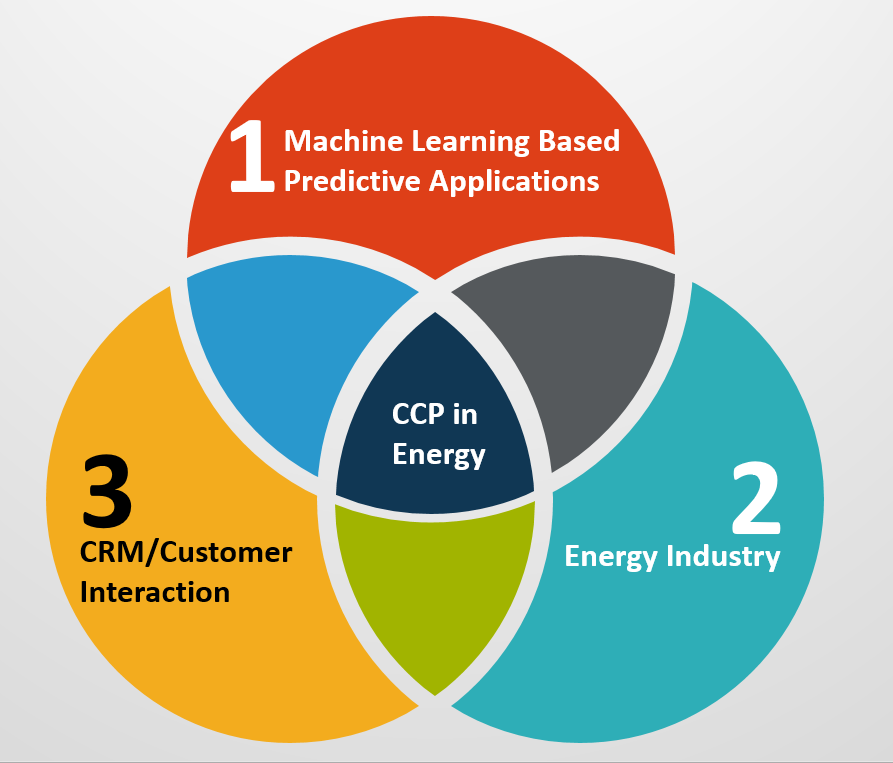
\includegraphics[width=0.5\textwidth]{Thesis-Research-Area.png}
    \centering
    \caption{Thesis research area}
    \label{fig:research-area}
\end{figure}

\section{Research questions and objectives}

The primary goal of this thesis is to accurately predict the future churn or status of costumers (stays/churns) for an Italian energy supply company for the next 2 months. Machine learning is the tool that will be used to achieve our goal. Thereby, a theoretical overview of related machine learning concepts is needed in order to create a good model. The obtained models are compared using some metrics an the best performing one is selected to be used in production. Based on these objectives he following research questions are formulated:

\begin{enumerate}
	\item What is the current state of costumer churn prediction in the 			literature?
  	\item What is the current state of costumer churn prediction on the energy supply field?
  	\item Which models can be used to accurately predict costumer churn given customer feature data in energy supply filed?
  	\item How can they be evaluated?
  	\item How different models compare to one another?
\end{enumerate}

\section{Methodology}

The study made in this thesis consisted in three steps. Foremost, some research are formulated based on the desired outcome and the literature. As a first part, we conducted general overview of the machine learning concepts that are necessary to fully understand this thesis. The second part consisted in searching the literature to find related work that were used as inspiration for the last part. Finally, starting from the literature review, we selected some \gls{ML} models and some evaluations metrics to build a churn predictive application.

Data was provided by an Italian energy provider and consisted in real costumer data from May 2019 to June 2020. Unfortunately, for privacy reasons the data cannot be disclosed alongside this thesis.

\section{Structure of the thesis}

The second chapter presents a high level overview of critical methodologies and concepts useful to understand the study performed in this thesis. In the third chapter we perform a review of related existing studies in the field of customer churn prediction. Next, in the fourth chapter an empirical study is conducted to prepare the data and build the churn prediction machine learning model. In chapter five we analyze the model results. Finally in chapter six, we discuss the results, eventual limitations, make the conclusions along with the proposals for future studies on the topic.

\chapter{Machine learning: Some theoretical concepts}



\section{Data collection and preprocessing}

The page is fixed at the dimensions of an A4 paper, therefore you have to print your thesis on A4 paper to obtain the best results. The font dimension

\subsection{ETL}

The page is fixed at the dimensions of an A4 paper, therefore you have to print your thesis on A4 paper to obtain the best results. The font dimension

\subsection{Apache spark}

The page is fixed at the dimensions of an A4 paper, therefore you have to print your thesis on A4 paper to obtain the best results. The font dimension

\subsection{Dealing with missing data}

The page is fixed at the dimensions of an A4 paper, therefore you have to print your thesis on A4 paper to obtain the best results. The font dimension

\subsection{Dealing with imbalance data}

The page is fixed at the dimensions of an A4 paper, therefore you have to print your thesis on A4 paper to obtain the best results. The font dimension

\subsection{One hot encoding}

The page is fixed at the dimensions of an A4 paper, therefore you have to print your thesis on A4 paper to obtain the best results. The font dimension

\subsection{Ordinal encoding}

The page is fixed at the dimensions of an A4 paper, therefore you have to print your thesis on A4 paper to obtain the best results. The font dimension

\subsection{Word embedding}

The page is fixed at the dimensions of an A4 paper, therefore you have to print your thesis on A4 paper to obtain the best results. The font dimension

\subsection{Data Normalization}

The page is fixed at the dimensions of an A4 paper, therefore you have to print your thesis on A4 paper to obtain the best results. The font dimension

\subsection{Feature selection}

The page is fixed at the dimensions of an A4 paper, therefore you have to print your thesis on A4 paper to obtain the best results. The font dimension


\section{Machine learning models}

The captions have a smaller font respect to the text and the label is in boldface. The appearance of the margin notes has been improved.

\subsection{Logistic regression}

The captions have a smaller font respect to the text and the label is in boldface. The appearance of the margin notes has been improved.

\subsection{Random forest classifier}

The captions have a smaller font respect to the text and the label is in boldface. The appearance of the margin notes has been improved.

\subsection{Gradient-boosted tree classifier}

The captions have a smaller font respect to the text and the label is in boldface. The appearance of the margin notes has been improved.

\subsection{Decision tree classifier}

The captions have a smaller font respect to the text and the label is in boldface. The appearance of the margin notes has been improved.

\subsection{Support vector machine}

The captions have a smaller font respect to the text and the label is in boldface. The appearance of the margin notes has been improved.

\subsection{Multilayer perceptron}

The captions have a smaller font respect to the text and the label is in boldface. The appearance of the margin notes has been improved.


\section{Evaluation metrics}

As regards the image formats, please use vector images as much as possible! Use jpg images only for photographs! pdf\LaTeX\ supports the pdf, jpg and png formats.

\subsection{Confusion matrix}

The captions have a smaller font respect to the text and the label is in boldface. The appearance of the margin notes has been improved.

\subsection{Accuracy}

The captions have a smaller font respect to the text and the label is in boldface. The appearance of the margin notes has been improved.

\subsection{NDCG@K}

The captions have a smaller font respect to the text and the label is in boldface. The appearance of the margin notes has been improved.

\chapter{Related work}

In this chapter I will discuss my stylistic choices of \textsf{sapthesis}.
I will show the page layout geometry and I will describe the page style.

\section{Customer churn prediction}

The page is fixed at the dimensions of an A4 paper, therefore you have to print your thesis on A4 paper to obtain the best results. The font dimension

\section{Customer churn prediction in energy}

The page is fixed at the dimensions of an A4 paper, therefore you have to print your thesis on A4 paper to obtain the best results. The font dimension

\section{Summary}

The page is fixed at the dimensions of an A4 paper, therefore you have to print your thesis on A4 paper to obtain the best results. The font dimension

\chapter{Energy provider case study: churn prediction machine learning model}

The page is fixed at the dimensions of an A4 paper, therefore you have to print your thesis on A4 paper to obtain the best results. The font dimension

\section{Tools and libraries}

The page is fixed at the dimensions of an A4 paper, therefore you have to print your thesis on A4 paper to obtain the best results. The font dimension


\subsection{Python}

The page is fixed at the dimensions of an A4 paper, therefore you have to print your thesis on A4 paper to obtain the best results. The font dimension


\subsection{Apache Spark}

The page is fixed at the dimensions of an A4 paper, therefore you have to print your thesis on A4 paper to obtain the best results. The font dimension

\section{Data description and understanding}

The page is fixed at the dimensions of an A4 paper, therefore you have to print your thesis on A4 paper to obtain the best results. The font dimension

\section{Data preprocessing and feature selection}

The page is fixed at the dimensions of an A4 paper, therefore you have to print your thesis on A4 paper to obtain the best results. The font dimension

\subsection{Handling missing data}

The page is fixed at the dimensions of an A4 paper, therefore you have to print your thesis on A4 paper to obtain the best results. The font dimension

\subsection{Dealing with categorical features}

The page is fixed at the dimensions of an A4 paper, therefore you have to print your thesis on A4 paper to obtain the best results. The font dimension

\subsection{Imbalanced data}

The page is fixed at the dimensions of an A4 paper, therefore you have to print your thesis on A4 paper to obtain the best results. The font dimension

\subsection{Data Normalization}

The page is fixed at the dimensions of an A4 paper, therefore you have to print your thesis on A4 paper to obtain the best results. The font dimension

\subsection{Feature selection}

The page is fixed at the dimensions of an A4 paper, therefore you have to print your thesis on A4 paper to obtain the best results. The font dimension

\chapter{Models and results}

The page is fixed at the dimensions of an A4 paper, therefore you have to print your thesis on A4 paper to obtain the best results. The font dimension

\section{Logistic regression}

The page is fixed at the dimensions of an A4 paper, therefore you have to print your thesis on A4 paper to obtain the best results. The font dimension

\section{Random forest classifier}

The page is fixed at the dimensions of an A4 paper, therefore you have to print your thesis on A4 paper to obtain the best results. The font dimension

\section{Gradient-boosted tree classifier}

The page is fixed at the dimensions of an A4 paper, therefore you have to print your thesis on A4 paper to obtain the best results. The font dimension

\section{Decision tree classifier}

The page is fixed at the dimensions of an A4 paper, therefore you have to print your thesis on A4 paper to obtain the best results. The font dimension

\section{Support vector machine}

The page is fixed at the dimensions of an A4 paper, therefore you have to print your thesis on A4 paper to obtain the best results. The font dimension

\section{Multilayer perceptron}

The page is fixed at the dimensions of an A4 paper, therefore you have to print your thesis on A4 paper to obtain the best results. The font dimension

\section{Summary and analysis of the results}

The page is fixed at the dimensions of an A4 paper, therefore you have to print your thesis on A4 paper to obtain the best results. The font dimension

\chapter{Conclusions}

\section{Conclusion}

The page is fixed at the dimensions of an A4 paper, therefore you have to print your thesis on A4 paper to obtain the best results. The font dimension

\section{Suggestions for future research}

The page is fixed at the dimensions of an A4 paper, therefore you have to print your thesis on A4 paper to obtain the best results. The font dimension

\backmatter

\cleardoublepage
\phantomsection % Give this command only if hyperref is loaded
\addcontentsline{toc}{chapter}{\bibname}
\begin{thebibliography}{9}

\bibitem{Geron2017} 
Aurélien Géron (13 March 2017). \href{https://books.google.com/books?id=bRpYDgAAQBAJ}{Hands-On Machine Learning with Scikit-Learn and TensorFlow: Concepts, Tools, and Techniques to Build Intelligent Systems}. O'Reilly Media. ISBN 978-1-4919-6224-4.

\bibitem{Sousa2015} 
Eusébio E., de Sousa J., Ventim Neves M. (2015). \href{https://doi.org/10.1007/978-3-319-16766-4_39}{Risk Analysis and Behavior of Electricity Portfolio Aggregator}. In: Camarinha-Matos L., Baldissera T., Di Orio G., Marques F. (eds) Technological Innovation for Cloud-Based Engineering Systems. DoCEIS 2015. IFIP Advances in Information and Communication Technology, vol 450. Springer, Cham.

\bibitem{Garcia2016} 
Martínez García I.E., Sánchez A.S., Barbati S. (2016). \href{https://doi.org/10.1007/978-3-319-39095-6_15}{Reliability and Preventive Maintenance}. In: Ostachowicz W., McGugan M., Schröder-Hinrichs JU., Luczak M. (eds) MARE-WINT. Springer, Cham.

\end{thebibliography}

\end{document}